\documentclass{beamer}

\mode<presentation> {
\usetheme[secheader]{Madrid}
\usecolortheme{seahorse}
\useinnertheme{circles}
}

\usepackage{graphicx} % Allows including images
\usepackage{booktabs} % Allows the use of \toprule, \midrule and \bottomrule in tables
\usepackage{tikz}
\usepackage{url}


%----------------------------------------------------------------------------------------
%	TITLE PAGE
%----------------------------------------------------------------------------------------

\title[Modeling]{Modeling} % The short title appears at the bottom of every slide, the full title is only on the title page

\author{Chaklam Silpasuwanchai} % Your name
\institute[AIT] % Your institution as it will appear on the bottom of every slide, may be shorthand to save space
{
Asian Institute of Technology \\ % Your institution for the title page
\medskip
\textit{chaklam@ait.asia} % Your email address
}
\date{} % Date, can be changed to a custom date

\AtBeginSection[]
{
\begin{frame}<beamer> 
\tableofcontents[currentsection]  % show TOC and highlight current section
\end{frame}
}

\begin{document}

\begin{frame}
\titlepage % Print the title page as the first slide
\end{frame}

\begin{frame}
\frametitle{Overview} % Table of contents slide, comment this block out to remove it
\tableofcontents % Throughout your presentation, if you choose to use \section{} and \subsection{} commands, these will automatically be printed on this slide as an overview of your presentation
\end{frame}

%\begin{frame}
%	\frametitle{Reminders}
%	\begin{itemize}
%		\item Next week final exam, and then we shall find a day to present our final project.  Final exam covers everything from midterm onward.   Open book/internet.
%	\end{itemize}
%\end{frame}

%----------------------------------------------------------------------------------------
%	PRESENTATION SLIDES
%----------------------------------------------------------------------------------------

%------------------------------------------------

\begin{frame}
\frametitle{Sources} 
\begin{itemize}
	\item Mackenzie, Chapter 7, \textbf{Modeling Interaction},  Human Computer Interaction: An Empirical Research Perspective, 1st ed. (2013) 
\end{itemize}
\end{frame}

%\begin{frame}
%	\frametitle{Model}
%	\begin{itemize}
%		\item Model is a \textbf{simplification of reality}, allowing us to explore the phenomena, \textbf{without actually constructing the building or throwing the ball}.
%		\item Model is either descriptive or predictive
%		\begin{itemize}
%			\item \textbf{Descriptive}: describe phenomena
%			\item \textbf{Predictive}: using mathematical equations to predict phenomena
%		\end{itemize}
%	\end{itemize}
%	\begin{figure}
%		\centering
%		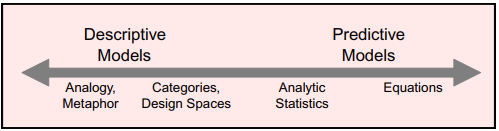
\includegraphics[width=0.7\linewidth]{image/7-42}
%		\caption{Source: Figure 7.42 (Mackenzie)}
%	\end{figure}
%\end{frame}

\begin{frame}
	\frametitle{Model}
	\begin{itemize}
		\item Model is a \textbf{simplification of reality}, allowing us to explore the phenomena, \textbf{without actually doing it}.
		\item Here we shall focus on three classic predictive models
		\begin{itemize}
			\item \textbf{Fitts' Law}: predict selection time
			\item \textbf{Choice reaction time}: predict reaction time given choices
			\item \textbf{Keystroke level model}: predict task completion time
%			\item \textbf{Skill acquisition}: predict skill gained
		\end{itemize}
	\end{itemize}
\end{frame}

%\section{Descriptive models}
%
%\subsection{Key-action model}
%\begin{frame}
%	\frametitle{Key-action model}
%	\begin{itemize}
%		\item With KAM, keyboard keys are categorized as either symbol keys, executive keys, or modifier keys.
%		\begin{enumerate}
%			\item \textbf{Symbol} keys deliver graphic symbols, e.g., letters, numbers %to an application 
%		%such as a text editor. These are typically letters, numbers, or punctuation symbols. 
%			\item  \textbf{Executive} keys invoke actions, e.g., Enter, F1, ESC% in the application or at the system level. 		
%			\item \textbf{Modifier} keys are modifiers, e.g., shift and alt
%		\end{enumerate}
%	\end{itemize}
%\end{frame}
%
%\begin{frame}
%	\footnotesize
%	\frametitle{Key-action model}
%	\begin{itemize}
%%		\item As you will see, the usage of descriptive model is simply allow us to delineates a problem space, and to identify any possible problem
%%		\item For example, consider the usage of left and right hands.  On the left, there are TAP, CAPS, ESC, and WINDOWS that are not mirrored.  On the right, there are at least 18 keys that are not mirrored, e.g., BACKSPACE, INSERT, DELETE, etc.  
%%		\item With a 4-18 left-right ratio of executive keys, the current desktop is clearly right-side bias!
%%		\item Given that the right hand is already occupied with the mouse, isn't the right hand too overloaded?
%%		\item In fact, research shows that common GUI tasks favor left-hand mouse usage! (Mackenzie, 2003)
%	\end{itemize}
%	\begin{figure}
%		\centering
%		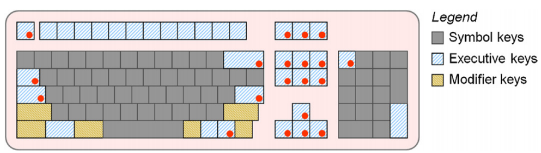
\includegraphics[width=0.5\linewidth]{image/7-3}
%		\caption{Source: Figure 7.3 (Mackenzie)}
%	\end{figure}
%\end{frame}
%
%\begin{frame}
%	\frametitle{Key-ambiguity model}
%	\begin{itemize}
%		\item The key-action model only captures one aspect of keyboards, namely the actions associated with each key.
%		\item Another way to think about keyboards is in the 
%		\textbf{ambiguity} of key presses. If pressing a symbol key always produces the same symbol, then the situation is simple. But if a key can produce two or more symbols, then this is worth thinking about.  
%		\item For this, a "key-ambiguity" descriptive model 
%		might be useful (MacKenzie and Soukoreff, 2002)
%		\item Optimal ambiguous keyboard would depend on the arrangement which is also dependent on ngrams
%	\end{itemize}
%	\begin{figure}
%		\centering
%		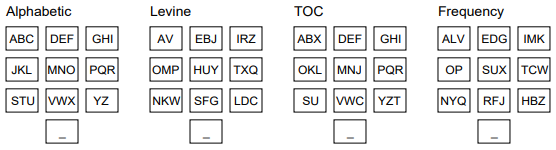
\includegraphics[width=0.5\linewidth]{image/1998}
%		\caption{Source: Lesher et al. 1998}
%	\end{figure}
%\end{frame}
%
%\subsection{Model of bi-manual control}
%
%\begin{frame}
%	\frametitle{Model of bi-manual control}
%	\begin{itemize}
%		\item Describes how we use our two hands in interaction
%		\item Guiard proposes a simple model, describing the logic of division of labor between the two hands
%		\item For example, a right-handed graphic artist is sketching, the left hand is used to manipulate the frame of workspace using coarse movement.  At the same time, the right hand follows the frame of workspace and sketching takes place using fine movements
%		\item Unsurprisingly, this model was widely adopted for HCI research in two-handed interaction
%	\end{itemize}
%	\begin{figure}
%		\centering
%		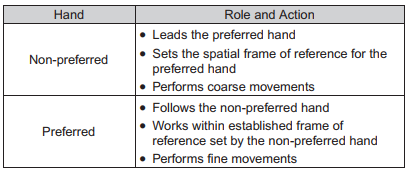
\includegraphics[width=0.5\linewidth]{image/7-4}
%		\caption{Source: Figure 7.4 (Mackenzie)}
%	\end{figure}
%\end{frame}
%
%\begin{frame}
%	\frametitle{Model of bi-manual control}
%	\begin{itemize}
%		\item Back then, \textbf{scrolling} is a time-consuming process where users have to acquire the scrollbar on the right, which is a target acquisition task that takes up \textbf{two seconds} per trial
%		\item Microsoft's \textbf{IntelliMouse} introduces new affordance in 1996, introducing a scrolling wheel
%		\item Guiard model informs us that indeed, it was a bad idea as left hand would be a much better idea.  Why?  Imagine scrolling while selecting - it's impossible with this design
%	\end{itemize}
%	\begin{figure}
%		\centering
%		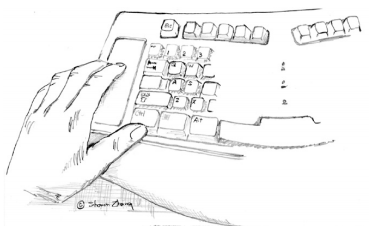
\includegraphics[width=0.4\linewidth]{image/7-7}
%		\caption{Source: Figure 7.7 (Mackenzie)}
%	\end{figure}
%\end{frame}
%
%\begin{frame}
%	\frametitle{Model of bi-manual control}
%	Two-handed interaction research is ongoing
%	\begin{figure}
%		\centering
%		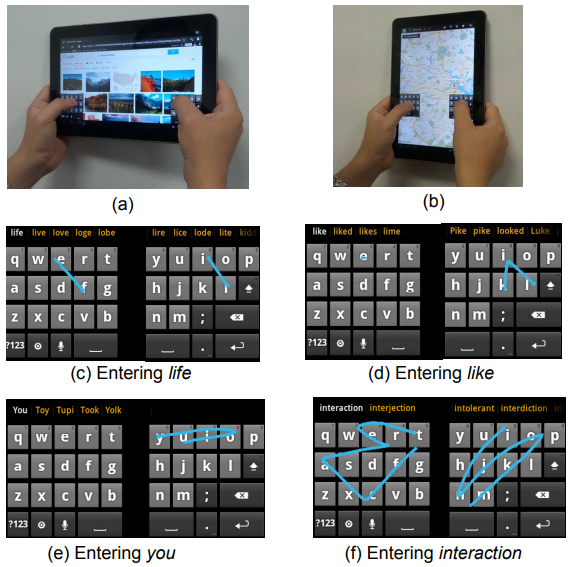
\includegraphics[width=0.6\linewidth]{image/xiaojuanbi}
%		\caption{Bi et al., \textbf{Bimanual Gesture Keyboard}, CHI 2012}
%	\end{figure}
%\end{frame}
%
%\begin{frame}
%	\frametitle{Model of bi-manual control}
%	Two-handed interaction research is ongoing
%	\begin{figure}
%		\centering
%		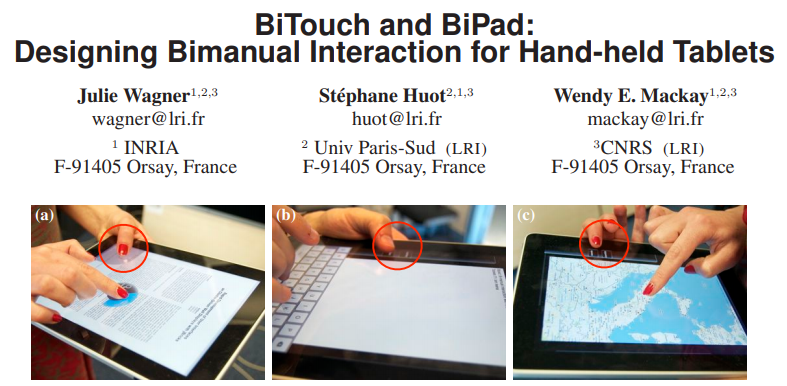
\includegraphics[width=0.9\linewidth]{image/wagner}
%		\caption{Wagner et al., \textbf{BiTouch and BiPad:
%				Designing Bimanual Interaction for Hand-held Tablets}, CHI 2012}
%	\end{figure}
%\end{frame}
%
%\subsection{Three-state model of graphical input}
%
%\begin{frame}
%	\frametitle{Three-state model of graphical input}
%	\begin{itemize}
%		\item Another descriptive model is \textbf{Buxton's three-state model of graphical input}
%		\item The model is a simple characterization of the operation of computer pointing devices in terms of \textbf{state transitions.}
%		\item Such simple model may seem obvious but its simplicity affords extension to multi-button interaction, stylus, or finger input.
%	\end{itemize}
%	\begin{figure}
%		\centering
%		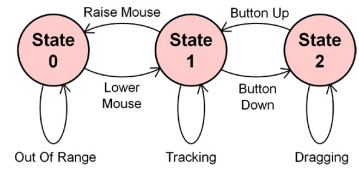
\includegraphics[width=0.5\linewidth]{image/7-9}
%		\caption{Source: Figure 7.9 (Mackenzie)}
%	\end{figure}
%\end{frame}
%
%\begin{frame}
%	\frametitle{Three-state model of graphical input}
%	\footnotesize
%	\begin{itemize}
%		\item Apple in 1994 commercialized a 
%		new pointing device in its PowerBook 500 notebook computer: the \textbf{Trackpad touchpad}
%		\item One of the interaction techniques supported by touchpads is "\textbf{lift-and-tap}" where primitive operations like clicking, double-clicking, and dragging are implemented without a button
%		\item Two observations follow: (1) lift-and-tap necessitates \textbf{	extra state transitions} over mouse, and (2) the use of state 1-0-1 transitions for lift-and-tap is confounded with clutching (lifting the mouse to reposition) which uses the same state transitions, thus possibly System enters the Tracking state instead of the Dragging state
%		\item To fix this, additional sensing capability was used to implement state 1-2 transitions by \textbf{pressing harder} or use \textbf{gestures}
%	\end{itemize}
%	\begin{figure}
%		\centering
%		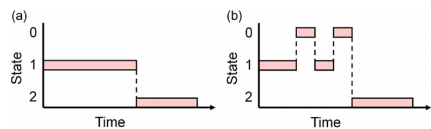
\includegraphics[width=0.6\linewidth]{image/7-10}
%		\caption{Source: Figure 7.10 (Mackenzie)}
%	\end{figure}
%\end{frame}

%\section{Predictive models}

%\begin{frame}
%	\frametitle{Predictive models}
%	\begin{itemize}
%		\item A predictive model is an equation, where predictors (x) predicts the outcome (y).  
%		\item Since it is an equation, both x and y use ratio-scale data.  For example, y cannot be nominal (categorical) as in the case of experimental design
%		\item Models in HCI has primary two purpose: (1) provides a mathematical explanation of the relationships between predictors and targets, (2) serve as a function for analyses of design alternatives
%		\item Simplest model in HCI comes in the form of a linear regression model
%	\end{itemize}
%\end{frame}

%\section{Linear regression model}
%
%\begin{frame}
%	\frametitle{Linear regression model}
%	\begin{figure}
%		\centering
%		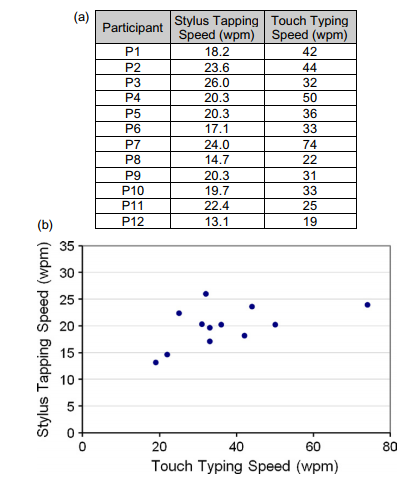
\includegraphics[width=0.6\linewidth]{image/7-12}
%		\caption{Source: Figure 7.12 (Mackenzie)}
%	\end{figure}
%\end{frame}
%
%\begin{frame}
%	\footnotesize
%	\frametitle{Linear regression model}
%	\begin{itemize}
%		\item 	\textit{R}$^{2}$\ is a common metric for linear regression model which measures the amount of variation that is explained by the model
%		\item Given 60wpm, the model predict stylus speed of 23.1wpm
%		\item SE = 3.39wpm.  Values within -1.96 SE and +1.96 SE of a prediction are within a 95\% confidence interval. So for the model developed here, there is 95\% confidence that a user whose touch-typing speed is 60wpm will have a stylus-tapping speed between 23.1 - (1.96 * 3.39) = 16.4wpm and 23.1 + (1.96 * 3.39) = 29.7wpm
%	\end{itemize}
%	\begin{figure}
%		\centering
%		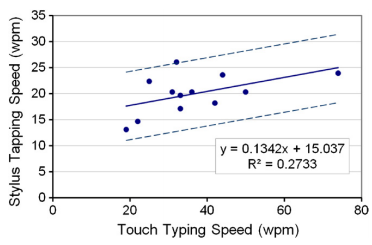
\includegraphics[width=0.4\linewidth]{image/7-13}
%		\caption{Source: Figure 7.13 (Mackenzie)}
%	\end{figure}
%\end{frame}
%
%\begin{frame}
%	\frametitle{More than one predictor}
%	\begin{itemize}
%		\item Prediction model can include \textbf{multiple predictors} and come in the form of multiple regression as:
%		\item \textbf{Stepwise linear regression} is commonly used
%	\end{itemize}
%	\centering
%	$y = a + b_{1}x_{1} + b_{2}x_{2} + b_{3}x_{3} + ...$
%	\begin{figure}
%		\centering
%		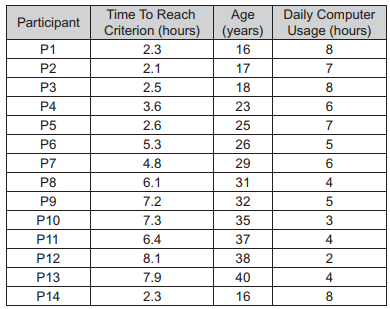
\includegraphics[width=.50\linewidth]{image/7-39}
%		\caption{Source: Figure 7.39 (Mackenzie)}
%	\end{figure}
%\end{frame}

\section{Fitts' Law}
\begin{frame}
	\frametitle{Fitts' Law}
	One of the most widely used models in HCI is Fitts’ law (1954).  Three primary usage are
	\begin{itemize}
		\item To see if the interaction technique follows Fitts' law
		\item To analyze design alternatives
		\item To use Fitts' index of performance (now throughput) as a dependent variable in a comparative evaluation
	\end{itemize}
	\begin{figure}
		\centering
		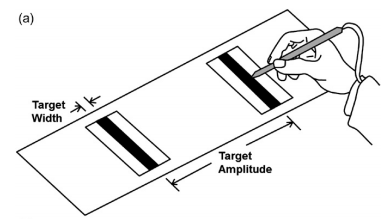
\includegraphics[width=0.5\linewidth]{image/7-14}
		\caption{Source: Figure 7.14 (Mackenzie)}
	\end{figure}
\end{frame}

\begin{frame}
	\footnotesize
	\frametitle{Fitts' Law}
		\centering
		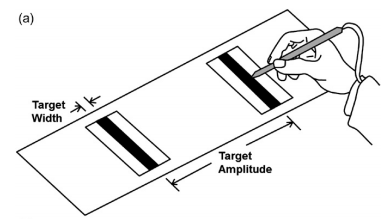
\includegraphics[width=0.4\linewidth]{image/7-14}
		\begin{itemize}
		\item Fitts proposed a variable quantifying movement task's difficulty - \textit{ID}, \textit{the index of difficulty}.
	\end{itemize}
	\centering
	$ID = log_{2}\left ( \frac{A}{W} + 1 \right )$
	\begin{itemize}
		\item To use Fitts law to predict MT, it is a linear function of ID where a and b are obtained from experiments
	\end{itemize}
	\centering
	$MT = a + b * ID$
	\begin{itemize}
		\item Fitts' index of performance, now called throughput (TP, in bits/s), is calculated as
	\end{itemize}
	\centering
	$TP = \left ( \frac{ID}{MT} \right )$
\end{frame}

\begin{frame}
	\frametitle{Improved Fitts' Law}
	\begin{itemize}
		\item Crossman (1956) proposed new \textbf{effective target width} ($W_e$).  $W_e$ is computed from the \textbf{standard deviation} in the selection coordinates gathered over a sequence of trials for a particular A-W condition.   If the selections are logged as x coordinates along the axis of approach to the target, then %$W_e$ is computed from the standard deviation in the selection coordinates gathered over a sequence of trials for a particular D-W condition. 
	\end{itemize}
	\centering
	$W_{e} = 4.133 * SD_{x}$
	\begin{itemize}
		\item hence
	\end{itemize}
	\centering
	$ID_e = log_{2}\left ( \frac{A}{W_e} + 1 \right )$
	\begin{itemize}
		\item hence
	\end{itemize}
	\centering
	$TP = \left ( \frac{ID_{e}}{MT} \right )$
\end{frame}

\begin{frame}
	\frametitle{Example}
	\begin{figure}
		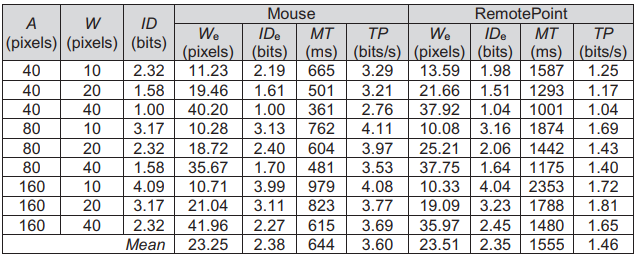
\includegraphics[width=1\linewidth]{image/7-16}
		\caption{Figure 7.16 (Mackenzie)}
	\end{figure}
\end{frame}

\begin{frame}
	\frametitle{Example}
	\begin{figure}
		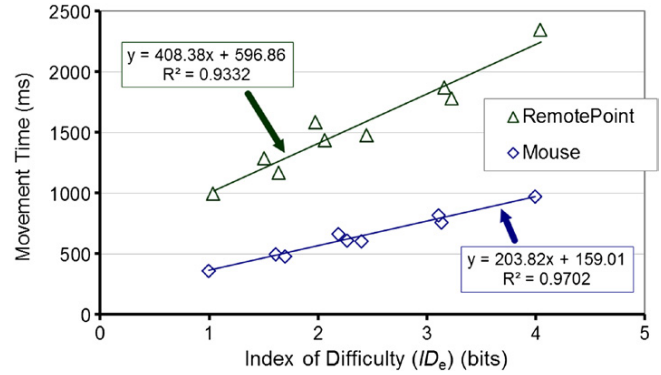
\includegraphics[width=0.8\linewidth]{image/7-17}
		\caption{Figure 7.17 (Mackenzie)}
	\end{figure}
\end{frame}

\begin{frame}
	\frametitle{Fitts' Law}
	\begin{itemize}
		\item By using Fitts' law as objective/cost function, we can find optimal design alternatives - an area called \textbf{design optimization}
	\end{itemize}
	\centering
	\begin{figure}
		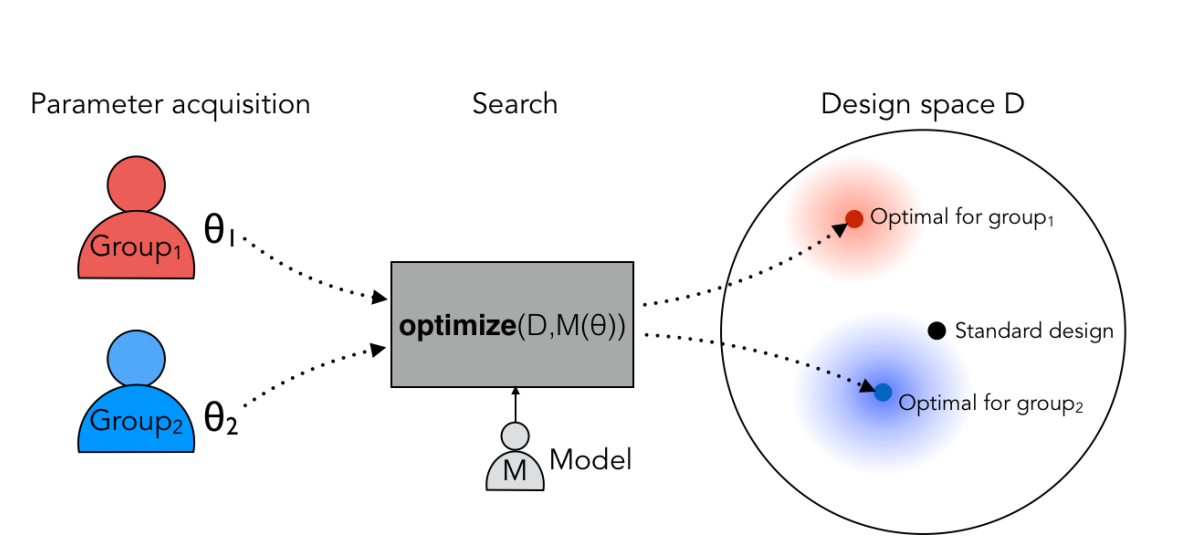
\includegraphics[width=.9\linewidth]{image/optimization}
		\caption{Source: Sarcar et al., \textbf{Ability-Based Optimization of Touchscreen Interactions}, IEEE Pervasive}
	\end{figure}
\end{frame}

\begin{frame}
	\frametitle{Activities}
	\begin{block}{Classwork}
		Recall that we did a 1D Fitts task in the previous class.   Use the data and (1) calculate ID, (2) plot the linear model with the equation and (3) calculate the $R^2$. You can use Excel or any spreadsheet diagram. 
	\end{block}
\end{frame}

\section{Choice reaction time}

\begin{frame}
	\frametitle{Hick-Hyman Law}
	\begin{itemize}
		\item Given $n$ stimuli, associated one-for-one with $n$ responses, the time to react ($RT$) to the onset of a stimulus is given by,
	\end{itemize}
		\centering
		$RT = a + b * log_{2}\left ( n + 1 \right )$
		\vspace{3pt}
	\begin{itemize}
		\item where $a$ and $b$ are empirically determined constants.  Typical values for $a$ is 200ms and $b$ is 150ms/bit
 	\end{itemize}		
	\begin{figure}
		\centering
		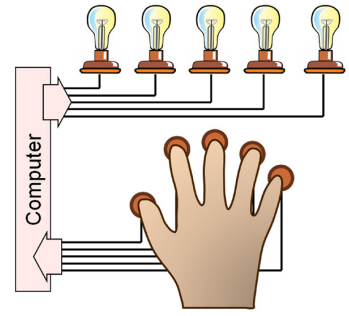
\includegraphics[width=.3\linewidth]{image/7-18}
		\caption{Source: Figure 7.18 (Mackenzie)}
	\end{figure}
\end{frame}

\begin{frame}
	\frametitle{Hick-Hyman Law}
	\begin{itemize}
		\item If \textbf{some choice is more probable than others}, this reduces the information content, thus in turn reduces the choice reaction time
		\item For a set of alternatives with different probabilities, the information load H is 
	\end{itemize}
	\centering
	$H = \sum p_{i}log_{2}\left ( \frac{1}{p_{i}} + 1 \right )$
	\begin{itemize}
		\item Consider a choice selection task where the choice is among 26 alternatives and all appear with equal probability, the information content of the task is simply
	\end{itemize}
	$H = log_{2}\left ( 27 \right ) = 4.75 bits$
\end{frame}

\begin{frame}
	\frametitle{Hick-Hyman Law}
	\begin{figure}
		\centering
		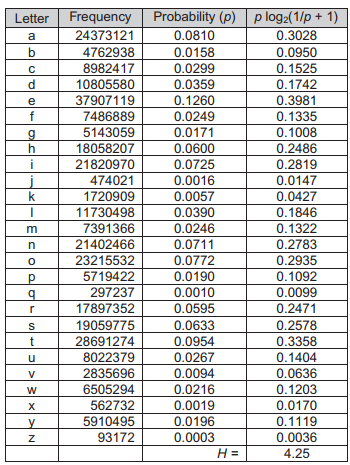
\includegraphics[width=.4\linewidth]{image/7-19}
		\caption{Source: Figure 7.19 (Mackenzie)}
	\end{figure}
\end{frame}

\begin{frame}
	\frametitle{Hick-Hyman Law}
	\begin{itemize}
		\item Card et al. (1983, 74) describe an example of a \textbf{telephone operator} selecting among ten buttons
		\item Landauer and Nachbar (1985) applied the Hick-Hyman law in measuring and predicting the time to select items in \textbf{hierarchical menus}%breadth should be favored over depth in hierarchical menus (\textit{Note that choice reaction is different from visual search, which is 
		%a linear function of the number of items. Landauer and Nachbar eliminated visual scanning in the task by ensuring that "the sets of choice alternatives were well practiced and well-ordered"})
		\item Ruiz et al. (2008) used the Hick-Hyman law to model the perception, planning, and activation time for users to \textbf{switch modes with their non-dominant hands} in a tablet interface
	\end{itemize}
\end{frame}

\begin{frame}
\frametitle{Activities}
\begin{block}{Example}
	\footnotesize
	A human operator attends to eight stimulus lights and presses one of eight keys when the corresponding light turns on. Two of the lights turn on more frequently than the others, accounting for 40 percent and 30 percent of all activations, respectively. The other lights activate with the same frequency. What is the information content of the task?
\end{block}
\end{frame}

\begin{frame}
\frametitle{Activities}
\begin{block}{Example}
	\footnotesize
	Below are the layouts for the Qwerty and Dvorak keyboards, as well as an alphabetic layout proposed by Card et al. (1983, 63). Assuming the layouts are implemented as standard physical keyboards, which design provides the most even split between lefthand and righthand keying?
\end{block}
	\begin{figure}
		\centering
		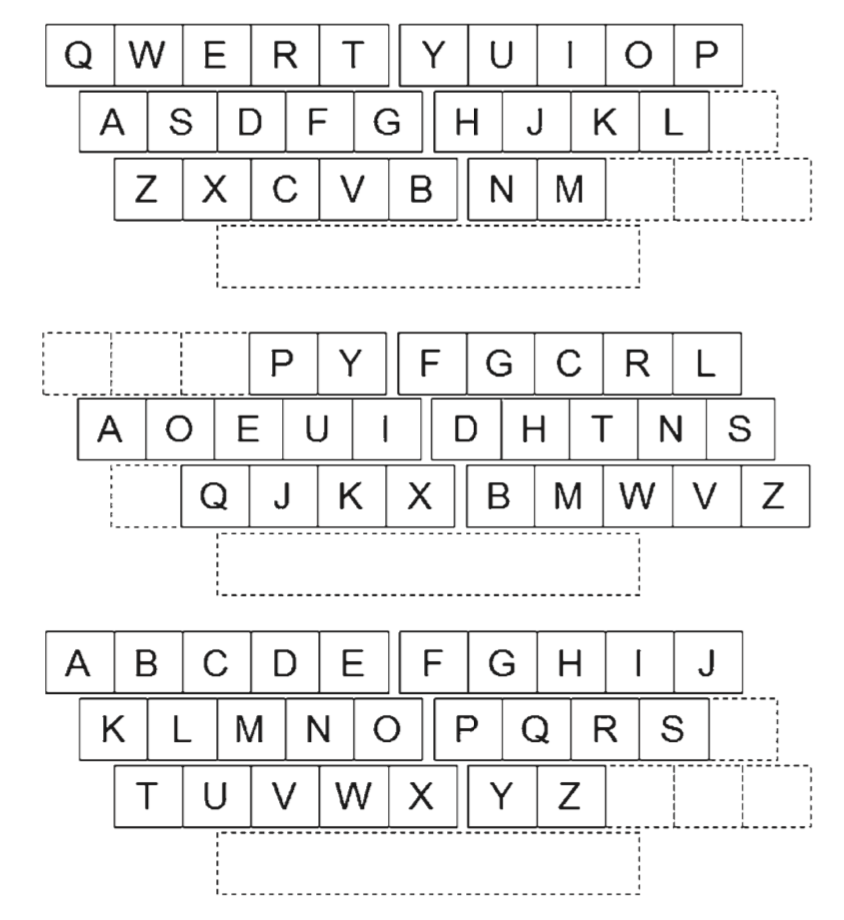
\includegraphics[width=.3\linewidth]{image/leftright}
	\end{figure}
\end{frame}

\section{Keystroke level model}

\begin{frame}
	\frametitle{Keystroke level model}
	\begin{itemize}
		\item Card et al. (1980; 1983, ch. 8) developed KLM that predict \textbf{error-free task completion time} 
%		using
%		\begin{itemize}
%			\item Task
%			\item Method used
%			\item Command language of the system
%			\item Motor skill parameters of the user
%			\item Response time parameters of the system
%		\end{itemize}
		\item The models works with four motor-control operators (K = keystroking, P = pointing, H = homing, D = drawing), one mental operator (M), and one system response operator (R):)
	\end{itemize}
	\centering
	$t_{EXECUTE} = t_{k} + t_{p} + t_{H} + t_{D} + t_{M} + t_{R}$
\end{frame}

\begin{frame}
	\frametitle{Keystroke level model}
	\centering
	Note that \textbf{empirical parameters can be updated}
	\begin{figure}
		\centering
		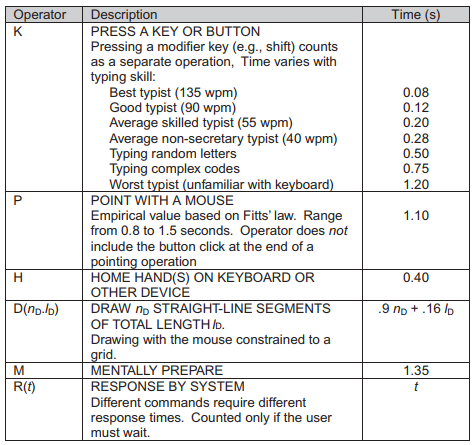
\includegraphics[width=.5\linewidth]{image/7-20}
		\caption{Source: Figure 7.20 (Mackenzie)}
	\end{figure}
\end{frame}

\begin{frame}
%	\footnotesize
	\frametitle{Keystroke level model}
	\begin{itemize}
%		\item To validate the KLM, Card, Moran, and Newell conducted an experiment using 14 tasks performed using various methods
%		\item Task T1, for example, was "Replace one 5-letter word with another (one line from previous task)."
		\item On one system, POET, the required sequence of subtasks was:
	\end{itemize}
	\begin{figure}
		\centering
		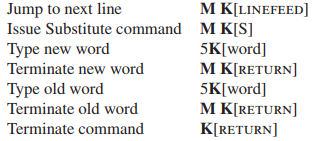
\includegraphics[width=.5\linewidth]{image/klm}
	\end{figure}
	\begin{itemize}
		\item The task required four mental operations (M) and 15 keystroking operations (K):
	\end{itemize}
	\centering
	$t_{EXECUTE} = 4 * t_{M} + 15 * t_{k} = 4 * 1.35 + 15 * 0.23 = 8.85s$
\end{frame}

\begin{frame}
	\centering
	Predicted and observed values are very close
	\frametitle{Keystroke level model}
	\begin{figure}
		\centering
		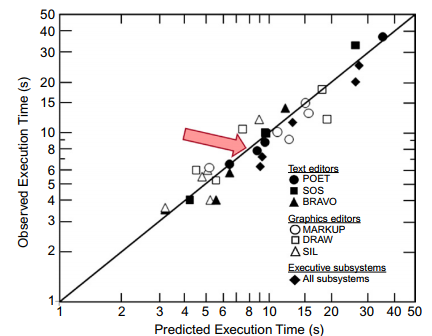
\includegraphics[width=.5\linewidth]{image/7-21}
		\caption{Source: Figure 7.21 (Mackenzie)}
	\end{figure}
\end{frame}

%\begin{frame}
%	\footnotesize
%	\frametitle{Keystroke level model}
%	\begin{figure}
%		\centering
%		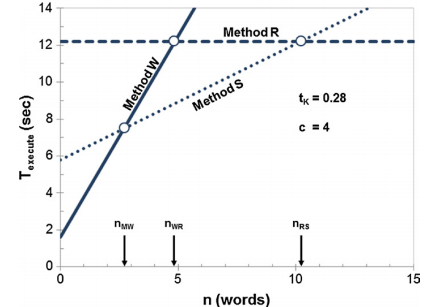
\includegraphics[width=.8\linewidth]{image/7-22}
%		\caption{Source: Figure 7.22 (Mackenzie)}
%	\end{figure}
%\end{frame}

%\begin{frame}
%	\frametitle{Keystroke level model}
%	\begin{itemize}
%		\item Note that \textbf{empirical parameters can be updated}.  For example, given the new mouse, we can recalculate $t_{p}$ given new obtained $a$ and $b$
%	\end{itemize}
%	\centering
%	$t_{p} = 0.159 + 0.204 * log_{2}\left ( \frac{A}{W} + 1 \right )$
%	\begin{itemize}
%		\item If we are clicking a 1.2cm wide toolbar button, and is 3.2cm away, the the pointing time is
%	\end{itemize}
%	\centering
%	$t_{p} = 0.159 + 0.204 * log_{2}\left ( \frac{3.2}{1.2} + 1 \right ) = 0.45s$
%	\begin{itemize}
%		\item Thus instead of 1.1s, our $t_{p}$ now equals 0.45 which is more accurate to nowadays
%	\end{itemize}
%\end{frame}

\begin{frame}
	\frametitle{Keystroke level model}
	\begin{itemize}
		\item Consider the editing operations to change the font style and font family for text, e.g., the word "M K"
		\item For mouse, four pointing operations are required: select the text, select the Bold, select the drop-down arrow in the Font list, and select Arial
		\item Table belows show KLM operators, where P is written in the format P[A, W].  The total time is
	\end{itemize}
	\centering
	$t_{EXECUTE} = 4 * t_{M} + \sum t_{p} = 4 * 1.35 + 2.71 = 8.11s $
	\begin{figure}
		\centering
		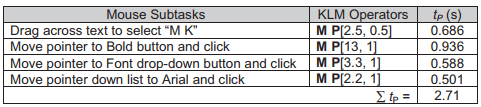
\includegraphics[width=.8\linewidth]{image/7-24}
		\caption{Source: Figure 7.24 (Mackenzie).  Note that P of Fitts' Law contains target selection as well, i.e., the click.}
	\end{figure}
\end{frame}

\begin{frame}
	\frametitle{Keystroke level model}
	\begin{itemize}
		\item The total time when using a keyboard is
	\end{itemize}
	\centering
	$t_{EXECUTE} = 4 * t_{M} + 12 * t_{k} = 4 x  1.35 + 12 x 0.75 = 14.40s $
	\begin{figure}
		\centering
		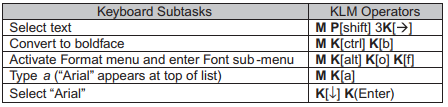
\includegraphics[width=.8\linewidth]{image/7-25}
		\caption{Source: Figure 7.25 (Mackenzie).   Typo note:  The first task should be M K[shift] 2K[$\rightarrow$].   Btw, why the last subtask doe not have a M operator?}
	\end{figure}
\end{frame}

%\begin{frame}
%	\frametitle{Keystroke level model}
%	\begin{itemize}
%		\item $t_{EXECUTE}$ in response to $t_{k}$
%	\end{itemize}
%	\begin{figure}
%		\centering
%		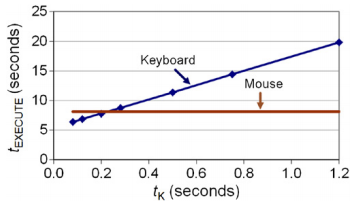
\includegraphics[width=.8\linewidth]{image/7-26}
%		\caption{Source: Figure 7.26 (Mackenzie)}
%	\end{figure}
%\end{frame}

%\begin{frame}
%	\frametitle{Keystroke level model}
%	KLM has been since extended for modern HCI research
%	\begin{itemize}
%		\item Ruiz et al. (2008) defined a new operator $t_{INT}$, the 
%		interval between a mode switch with the non-dominant hand and the beginning of the next action
%		\item Pettitt et al. (2007) define $t_RF$ for "reach far", the time to reach from a car's steering wheel to an IVIS (in-vehicle information system).
%		\item Whenever a extension of the model is proposed, an experiment is required to validate the extension
%		\item The key challenge lies in the $t_{k}$ which includes reacting, planning, pausing, and attending, and also lies in individual differences (novice vs. experts) which is the main limitation of the KLM model 
%		\item To tackle this limitation, HCI modeling is limited to primitive actions such as taps, clicks, gaze shifts, etc., instead of the whole execution time
%	\end{itemize}
%\end{frame}

%\begin{frame}
%	\frametitle{Keystroke level model}
%	\begin{itemize}
%		\item \textbf{Physical matching}: matching word
%		\item \textbf{Name matching}: same as physical matching but vary in  appearance, eg., uppercase/lowercase, font-size/family
%		\item \textbf{Class matching}: matching certain properties such as font-size/family
%	\end{itemize}
%	\begin{figure}
%		\centering
%		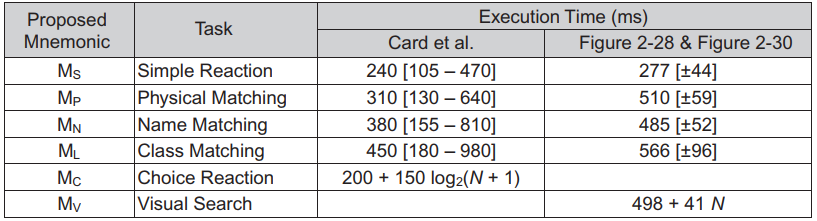
\includegraphics[width=.9\linewidth]{image/7-33}
%		\caption{Source: Figure 7.33 (Mackenzie)}
%	\end{figure}
%\end{frame}

%\begin{frame}
%	\footnotesize
%	\frametitle{Mobile text entry}
%	\begin{itemize}
%		\item KLM is a classic HCI example for \textbf{mobile text entry}
%		\item A relevant statistic is KSPC (\textbf{keystrokes per character}).  Typically, mobile phone has 
%		KSPC $\approx$ 2.023 for multi-tap and KSPC $\approx$ 1.007 for predictive text entry (T9)
%		\item If word completion or word prediction is added, KSPC $<$ 1. However, these figures do not account for the performance costs of\textbf{ visually attending} to the interface.
%		\item One important consideration in mobile text entry is the way users interaction with a phone either with a \textbf{thumb} or \textbf{index finger}
%		\item For touch typing on a Qwerty keyboard or multi-tapping on a mobile phone, \textbf{the KLM’s mental operator (M) is not needed}. The user knows what to do and does it according to his or her keystroking expertise with the method.
%		\item This is not the case for predictive text entry as it requires mental operations since uncertainty is present
%	\end{itemize}
%%	\begin{figure}
%%		\centering
%%		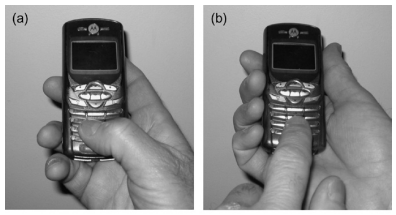
\includegraphics[width=.35\linewidth]{image/7-27}
%%		\caption{Source: Figure 7.27 (Mackenzie)}
%%	\end{figure}
%\end{frame}
%
%\begin{frame}
%	\frametitle{Mobile text entry}
%	\begin{figure}
%		\centering
%		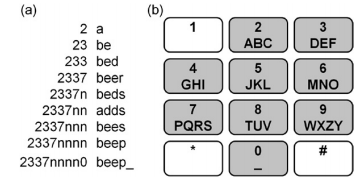
\includegraphics[width=.85\linewidth]{image/7-28}
%		\caption{Source: Figure 7.28 (Mackenzie)}
%	\end{figure}
%	\begin{figure}
%		\centering
%		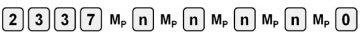
\includegraphics[width=.85\linewidth]{image/7-29}
%		\caption{Source: Figure 7.29 (Mackenzie)}
%	\end{figure}
%\end{frame}
%
%\begin{frame}
%	\frametitle{Predictive text entry}
%	Let's say "Vegetables".  Two possibilities of models are
%	\begin{figure}
%		\centering
%		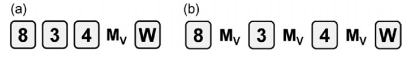
\includegraphics[width=.85\linewidth]{image/7-32}
%		\caption{Source: Figure 7.32 (Mackenzie)}
%	\end{figure}
%\end{frame}

%\section{Skill acquisition}
%
%\begin{frame}
%	\footnotesize
%	\frametitle{Skill acquisition}
%	\begin{itemize}
%		\item The relationship between \textbf{skill and practice is non-linear}. In the beginning, a small amount of practice yields substantial improvement. After a lot of practice, 
%		the same "small amount" produces only a slight improvement
%		\item This relationship can be written as below, where x is amount of practice and y is performance.
%	\end{itemize}
%	\centering
%	$y = b * x^{a}$
%	\begin{itemize}
%	\item If the dependent variable is the time to do a task, $T$, the equation can be rewritten as below, where $n$ is number of trial, and $T_{1}$ is the time on the first trial (\textit{Note that \textbf{a is negative} because completion time decreases over practice})
%	\end{itemize}
%	\centering
%	$T_{n} = T_{1} * n^{a}$
%	\begin{itemize}
%		\item Let's consider speed which takes a similar form, but \textbf{a is positive}, because speed increases over more practice)
%	\end{itemize}
%	\centering
%	$S_{n} = S_{1} * n^{a}$
%\end{frame}
%
%\begin{frame}
%	\footnotesize
%	\frametitle{Skill acquisition}
%	\begin{itemize}
%		\item Let's consider a comparison between two soft keyboard layouts: QWERTY and Opti
%		\item Since users are familiar with QWERTY, it is essential to perform a longitudinal study to understand the potential of Opti
%		\item The experiment involved 20 sessions of text entry
%	\end{itemize}
%	\begin{figure}
%		\centering
%		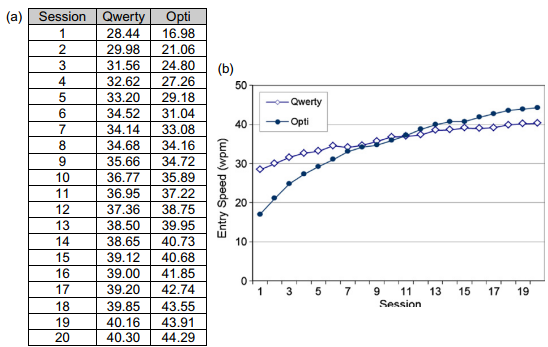
\includegraphics[width=.70\linewidth]{image/7-36}
%		\caption{Source: Figure 7.36 (Mackenzie)}
%	\end{figure}
%\end{frame}
%
%\begin{frame}
%	\frametitle{Skill acquisition}
%	For example, the speed after 50 trials are
%	\centering
%	$S_{50} = 17.24 * 50^{0.3219} = 60.7wpm$
%	\begin{figure}
%		\centering
%		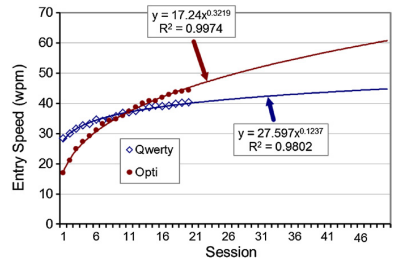
\includegraphics[width=.80\linewidth]{image/7-37}
%		\caption{Source: Figure 7.37 (Mackenzie)}
%	\end{figure}
%\end{frame}

\begin{frame}
	\frametitle{Activities}
	\begin{block}{Classwork}
		\footnotesize
		This task requires you to predict the time of mouse vs. keyboard using KLM.  For this ques­tion, assume $t_{K}$ = 0.4 seconds.    For $t_{P}$, use Figure 7.17 in previous slide where $x$ is $ID$.   Provide a KLM break­down of all operations for both mouse and keyboard.      Note that you don't have to worry about being exact,   rough reasonable estimates are ok.
		\begin{figure}
			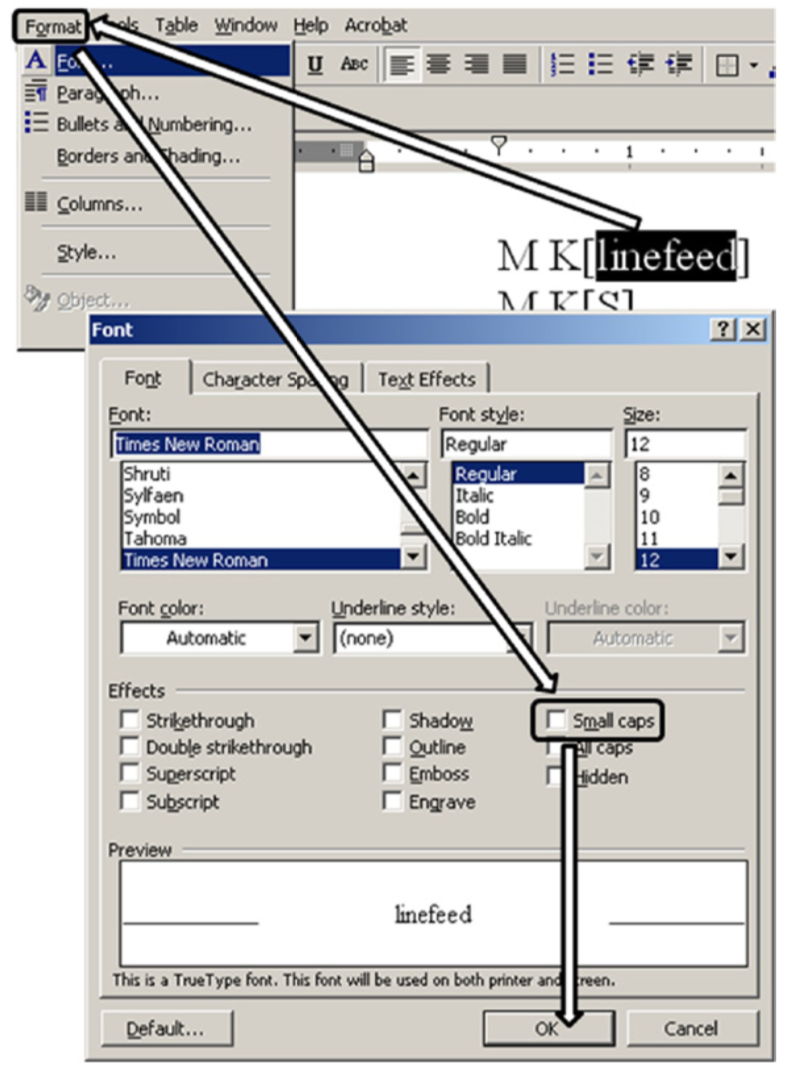
\includegraphics[width=.25\linewidth]{image/klm2}
		\end{figure}
	\end{block}
\end{frame}

%\begin{frame}
%\frametitle{Try it at home}
%\begin{block}{Try it at home}
%	\footnotesize
%-Download GoFitts.jar from \url{http://www.yorku.ca/mack/FittsLawSoftware}
%
%-Perform a 2D fitts tasks with default settings (A = 100, 200, 400; W = 20, 40, 80).
%
%-Set the Number of Trials to 5
%
%-Construct a table similar to below (Note that Mackenzie recommend using $ID_{e}$ as it accounts for both speed and accuracy)
%
%-Create a chart showing the
%a). scatter plot, 
%b). regression line, 
%c). R-squared, 
%d). prediction equation
%
%-Interpret the $R^{2}$ value.
%	\begin{figure}
%		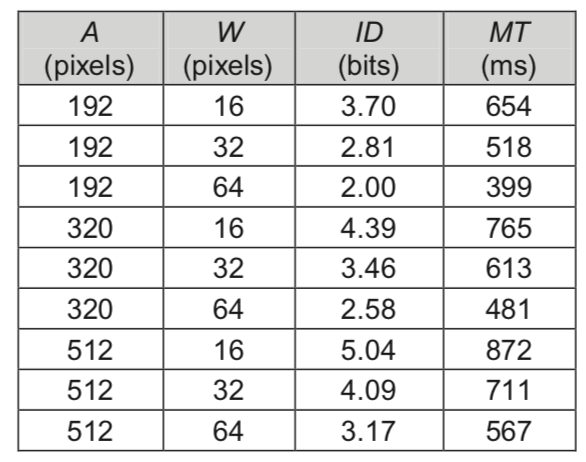
\includegraphics[width=.3\linewidth]{image/fitts}
%	\end{figure}
%\end{block}
%\end{frame}

%-----


%------------------------------------------------

%\begin{frame}
%\frametitle{Blocks of Highlighted Text}
%\begin{block}{Block 1}
%Lorem ipsum dolor sit amet, consectetur adipiscing elit. Integer lectus nisl, ultricies in feugiat rutrum, porttitor sit amet augue. Aliquam ut tortor mauris. Sed volutpat ante purus, quis accumsan dolor.
%\end{block}
%
%\begin{block}{Block 2}
%Pellentesque sed tellus purus. Class aptent taciti sociosqu ad litora torquent per conubia nostra, per inceptos himenaeos. Vestibulum quis magna at risus dictum tempor eu vitae velit.
%\end{block}
%
%\begin{block}{Block 3}
%Suspendisse tincidunt sagittis gravida. Curabitur condimentum, enim sed venenatis rutrum, ipsum neque consectetur orci, sed blandit justo nisi ac lacus.
%\end{block}
%\end{frame}

%------------------------------------------------

%\begin{frame}
%\frametitle{Multiple Columns}
%\begin{columns}[c] % The "c" option specifies centered vertical alignment while the "t" option is used for top vertical alignment
%
%\column{.45\textwidth} % Left column and width
%\textbf{Heading}
%\begin{enumerate}
%\item Statement
%\item Explanation
%\item Example
%\end{enumerate}
%
%\column{.5\textwidth} % Right column and width
%Lorem ipsum dolor sit amet, consectetur adipiscing elit. Integer lectus nisl, ultricies in feugiat rutrum, porttitor sit amet augue. Aliquam ut tortor mauris. Sed volutpat ante purus, quis accumsan dolor.
%
%\end{columns}
%\end{frame}

%------------------------------------------------
%\section{Second Section}
%%------------------------------------------------
%
%\begin{frame}
%\frametitle{Table}
%\begin{table}
%\begin{tabular}{l l l}
%\toprule
%\textbf{Treatments} & \textbf{Response 1} & \textbf{Response 2}\\
%\midrule
%Treatment 1 & 0.0003262 & 0.562 \\
%Treatment 2 & 0.0015681 & 0.910 \\
%Treatment 3 & 0.0009271 & 0.296 \\
%\bottomrule
%\end{tabular}
%\caption{Table caption}
%\end{table}
%\end{frame}

%------------------------------------------------

%\begin{frame}
%\frametitle{Theorem}
%\begin{theorem}[Mass--energy equivalence]
%$E = mc^2$
%\end{theorem}
%\end{frame}

%------------------------------------------------

%\begin{frame}[fragile] % Need to use the fragile option when verbatim is used in the slide
%\frametitle{Verbatim}
%\begin{example}[Theorem Slide Code]
%\begin{verbatim}
%\begin{frame}
%\frametitle{Theorem}
%\begin{theorem}[Mass--energy equivalence]
%$E = mc^2$
%\end{theorem}
%\end{frame}\end{verbatim}
%\end{example}
%\end{frame}

%------------------------------------------------

%\begin{frame}
%\frametitle{Figure}
%Uncomment the code on this slide to include your own image from the same directory as the template .TeX file.
%%\begin{figure}
%%\includegraphics[width=0.8\linewidth]{test}
%%\end{figure}
%\end{frame}

%------------------------------------------------

%\begin{frame}[fragile] % Need to use the fragile option when verbatim is used in the slide
%\frametitle{Citation}
%An example of the \verb|\cite| command to cite within the presentation:\\~
%
%This statement requires citation \cite{p1}.
%\end{frame}

%------------------------------------------------

%\begin{frame}
%\frametitle{References}
%\footnotesize{
%\begin{thebibliography}{99} % Beamer does not support BibTeX so references must be inserted manually as below
%\bibitem[Smith, 2012]{p1} John Smith (2012)
%\newblock Title of the publication
%\newblock \emph{Journal Name} 12(3), 45 -- 678.
%\end{thebibliography}
%}
%\end{frame}

%------------------------------------------------

\begin{frame}
\Huge{\centerline{Questions}}
\end{frame}

%----------------------------------------------------------------------------------------

\end{document} 
